\begin{frame}
\frametitle{Paging}

\begin{itemize}
  \item отображение VA на PA с гранулярностью в Page (блок память фиксированного размера);
  \item привелегии/права доступа проверяются на уровне страниц - меньше гранулярность;
  \item отображение описывается иерархической структурой (Page Table, далее PT) - большая гибкость;
  \item каждый процесс имеет свою PT - процессы изолированы друг от друга;
\end{itemize}
\end{frame}

\begin{frame}
\frametitle{Paging}
\framesubtitle{Таблицы страниц}

\begin{figure}
  \centering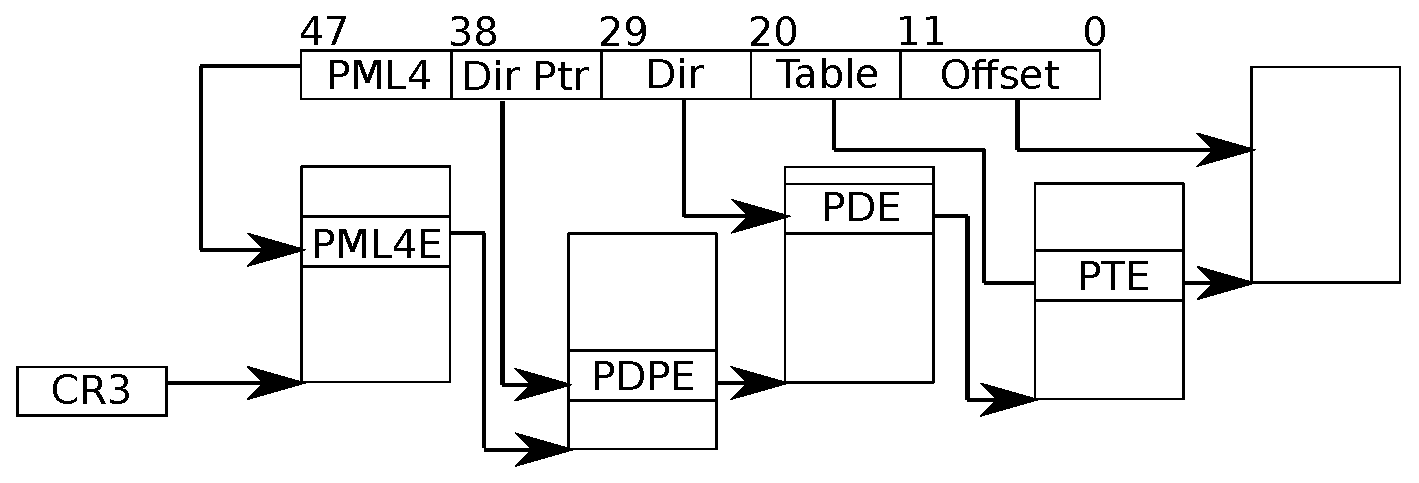
\includegraphics[width=.9\linewidth]{arch-page}
  \caption{x86-64 Page Tables}
\end{figure}
\end{frame}

\begin{frame}
\frametitle{Paging}
\framesubtitle{Права доступа и прочее}

\begin{itemize}
  \item Paging позволяет защитить память от доступа непривилегированного кода;
  \item Paging позволяет защитить память от доступа привилигерованного кода (SMEP/SMAP - защита kernelspace от атак из userspace);
  \item Paging позволяет запрещать исполнение кода в участке памяти;
  \item Paging позволяет управлять кешированием участка памяти;
  \item Paging вытеснил сегментацию (сегментация все еще используется в очень специфичных случаях);
\end{itemize}
\end{frame}

\begin{frame}
\frametitle{Paging}
\framesubtitle{Translation Lookaside Buffer}

\begin{itemize}
  \item<1-> Обращение к PT при каждом доступе к памяти - очень дорого
    \begin{itemize}
      \item чем больше памяти - тем больше уровней
      \item чем больше уровней - тем дороже трансляция
      \item чем больше памяти - тем медленее работа с ней (короче, все плохо)
    \end{itemize}
  \item<2-> Кеширование ускоряет процесс, но задача слишком специфичная - используем специальный кеш TLB;
  \item<3-> TLB не прозрачен для программиста - при изменении в PT нужно явно сбросить TLB;
\end{itemize}
\end{frame}

\begin{frame}
\frametitle{Page Fault}

Page Fault происходит если:
\begin{itemize}
  \item для виртуального адреса отсутствует отображение в физический (в x86 за это отвечает бит Present);
  \item отображение есть, но не достаточно прав доступа для обращения к памяти;
  \item произошла попытка записи в страницу только для чтения;
  \item произошла попытка исполнить кода со страницы не предназначенной для исполнения;
  \item обнаружена запись некорректного формата в PT;
\end{itemize}

\onslide<2->{Fault (в терминологии x86) - ошибка, которую можно исправить, виртуальный адрес по которому происходит обращение прилагается.}

\end{frame}

\begin{frame}
\frametitle{Page Fault}
\framesubtitle{On Demand Allocation}

\begin{figure}
  \centering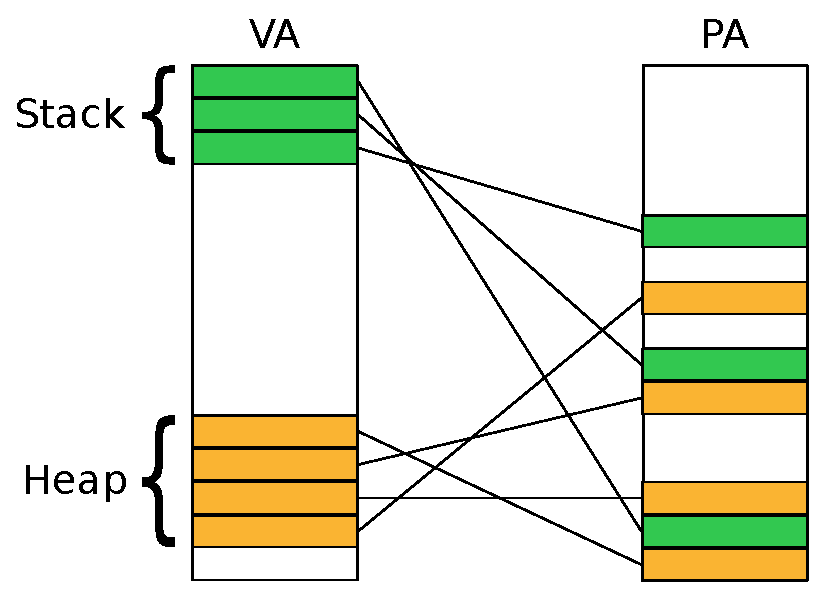
\includegraphics[width=.8\linewidth]{page-demand0}
  \caption{Отображение VA на PA}
\end{figure}
\end{frame}

\begin{frame}
\frametitle{Page Fault}
\framesubtitle{On Demand Allocation}

\begin{figure}
  \centering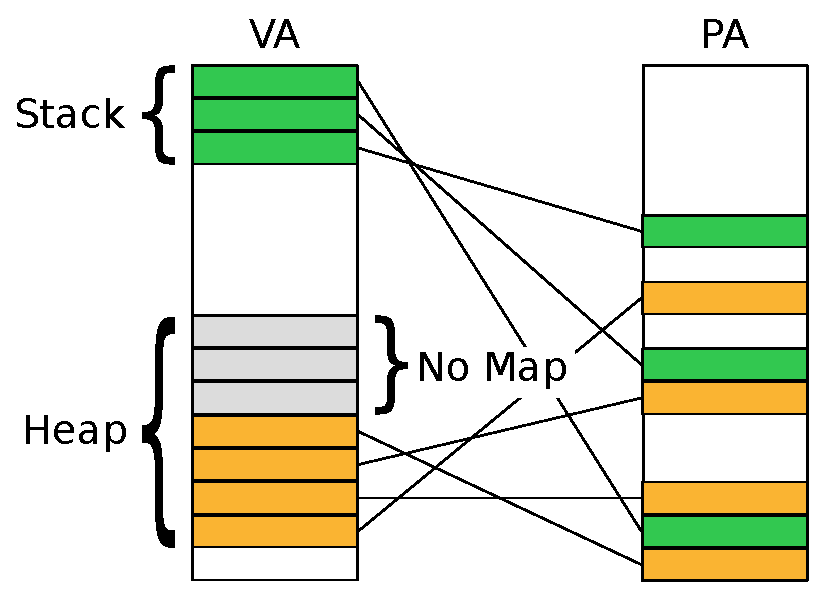
\includegraphics[width=.8\linewidth]{page-demand1}
  \caption{Процесс увеличвает Heap - страницы не выделяются}
\end{figure}
\end{frame}

\begin{frame}
\frametitle{Page Fault}
\framesubtitle{On Demand Allocation}

\begin{figure}
  \centering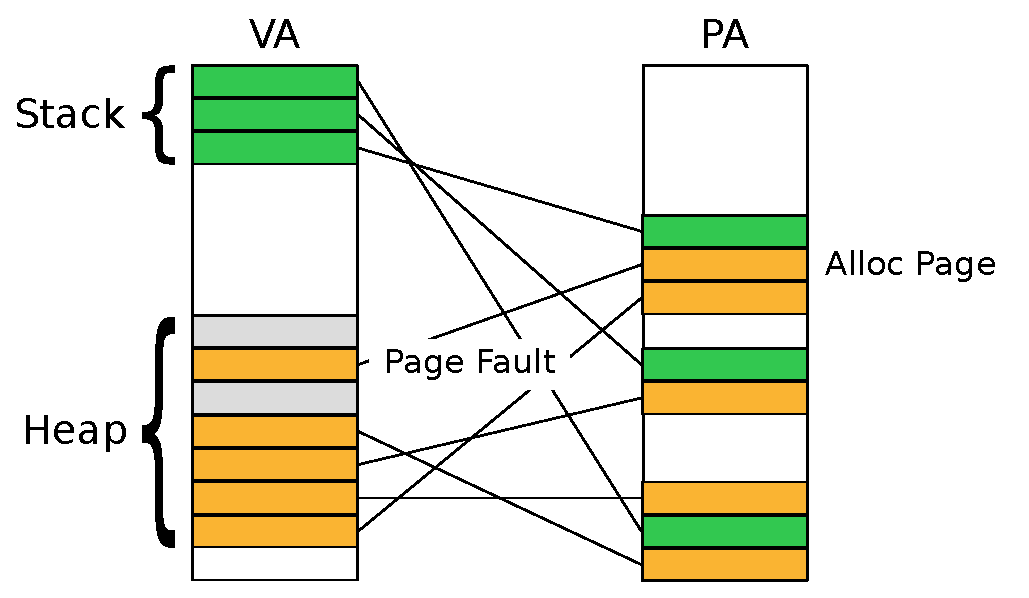
\includegraphics[width=.9\linewidth]{page-demand2}
  \caption{При робращении происходит Page Fault - выделяем страницу}
\end{figure}
\end{frame}

\begin{frame}
\frametitle{Page Fault}
\framesubtitle{On Demand Allocation}

\begin{itemize}
  \item<1-> аллоцируются только страницы, к котором происходит обращение - если процесс не использует память аллоцировать ее тоже не нужно;
  \item<2-> если ОС сказала, что аллоцировала память, еще не значит что она правда ее аллоцировала; \onslide<3->{с этим можно частично бороться:
    \begin{itemize}
      \item держать запас физических страниц для Page Fault;
      \item swapping может предотвратить самое худшее;
    \end{itemize}}
\end{itemize}
\end{frame}

\begin{frame}
\frametitle{Fork}
\framesubtitle{Копирование VA}

fork - системный вызов в Unix-like системах для создания нового процесса. Новый
процесс является копией старого. Т. е. нужно копировать VA:

\begin{itemize}
  \item честная копия VA может привести к большому количеству аллокаций физической памяти;
  \item честная копия VA может потребовать копирования большого количества памяти;
  \item<2-> честная копия, на самом деле, не нужна:
    \begin{itemize}
       \item не нужно копировать Read Only части VA;
       \item не нужно копировать то, что мы не будем использовать;
    \end{itemize}
\end{itemize}
\end{frame}

\begin{frame}
\frametitle{Page Fault}
\framesubtitle{Copy On Write}

\begin{figure}
  \centering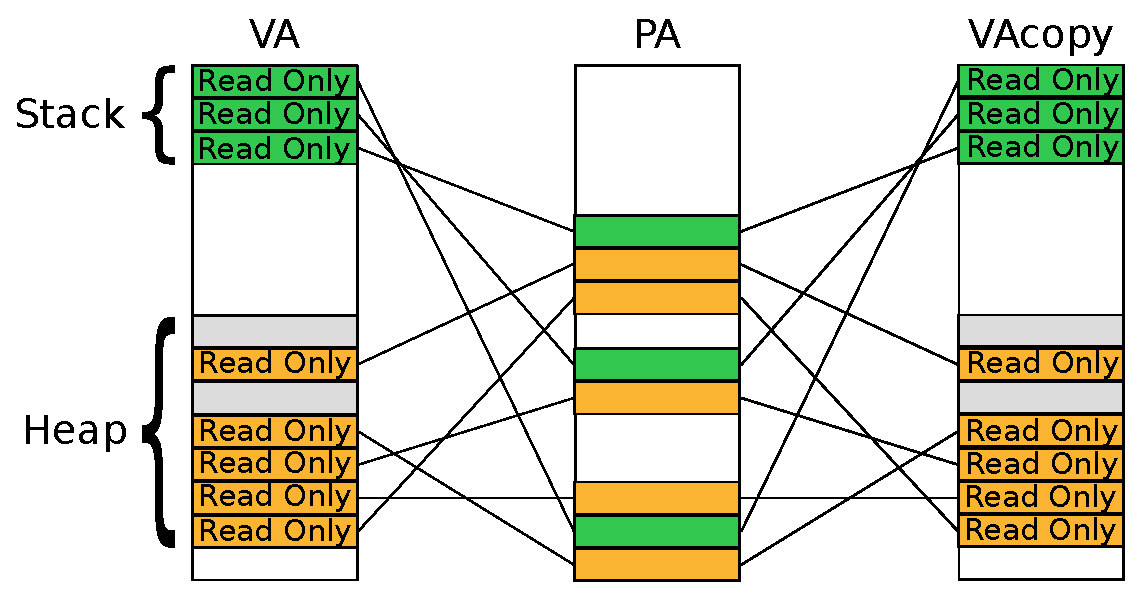
\includegraphics[width=.9\linewidth]{page-cow0}
  \caption{При копировании VA и оригинал и копия используют права Read Only}
\end{figure}
\end{frame}

\begin{frame}
\frametitle{Page Fault}
\framesubtitle{Copy On Write}

\begin{figure}
  \centering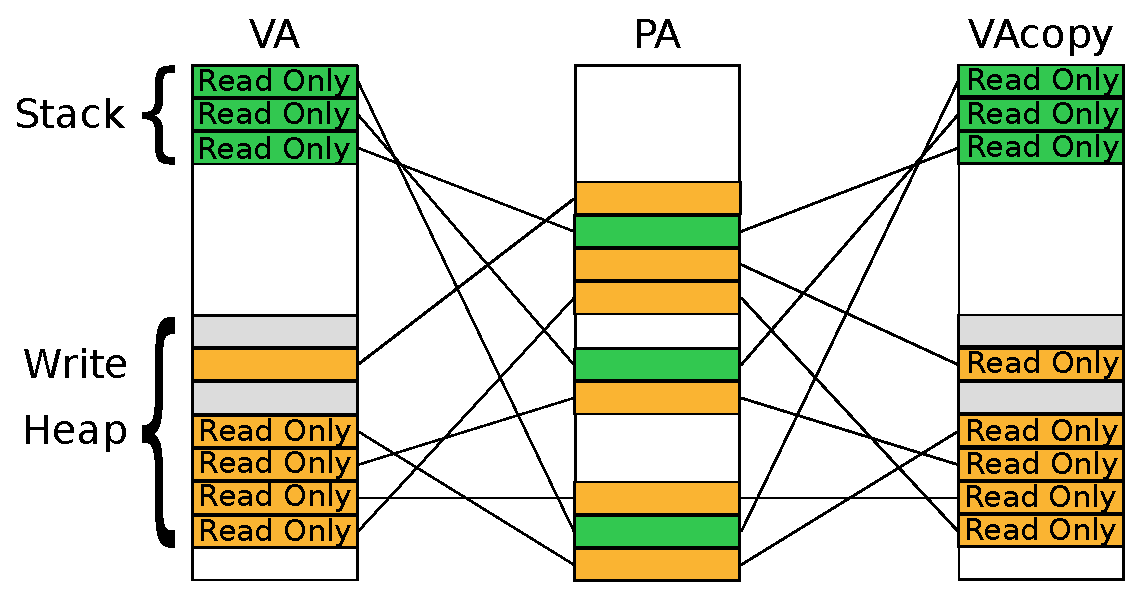
\includegraphics[width=.9\linewidth]{page-cow1}
  \caption{При записи происходит аллокация и настоящее копирование}
\end{figure}
\end{frame}

\begin{frame}
\frametitle{Page Fault}
\framesubtitle{Copy On Write}

\begin{figure}
  \centering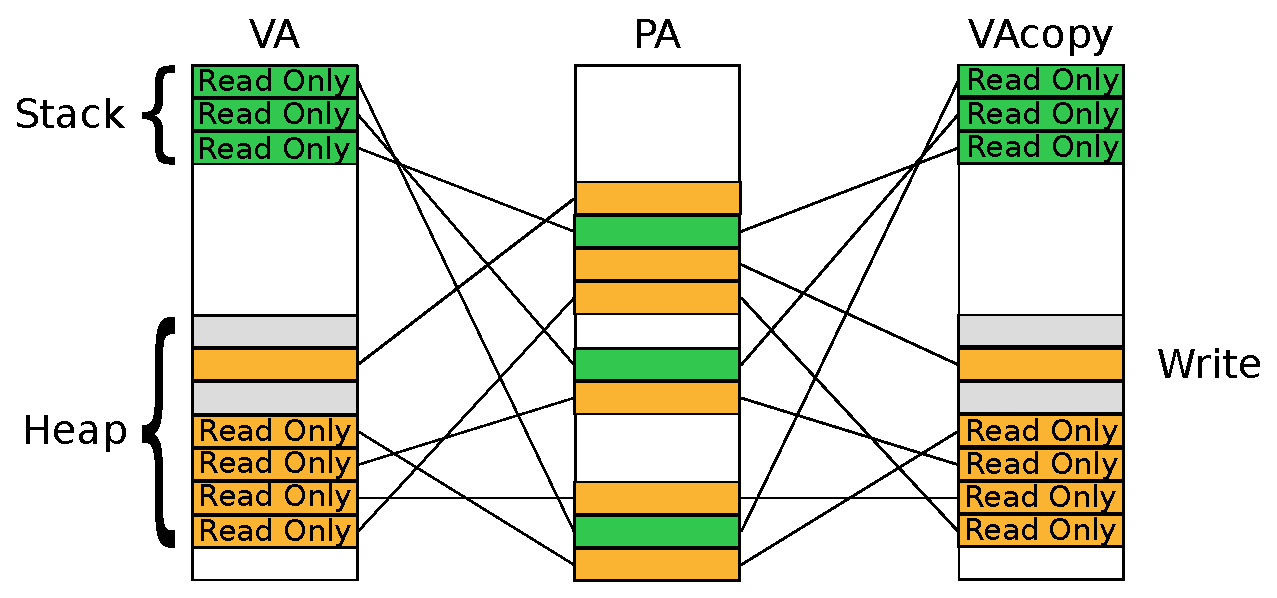
\includegraphics[width=.9\linewidth]{page-cow2}
  \caption{При записи происходит аллокация и настоящее копирование}
\end{figure}
\end{frame}

\begin{frame}
\frametitle{Page Fault}
\framesubtitle{Copy On Write}

\begin{figure}
  \centering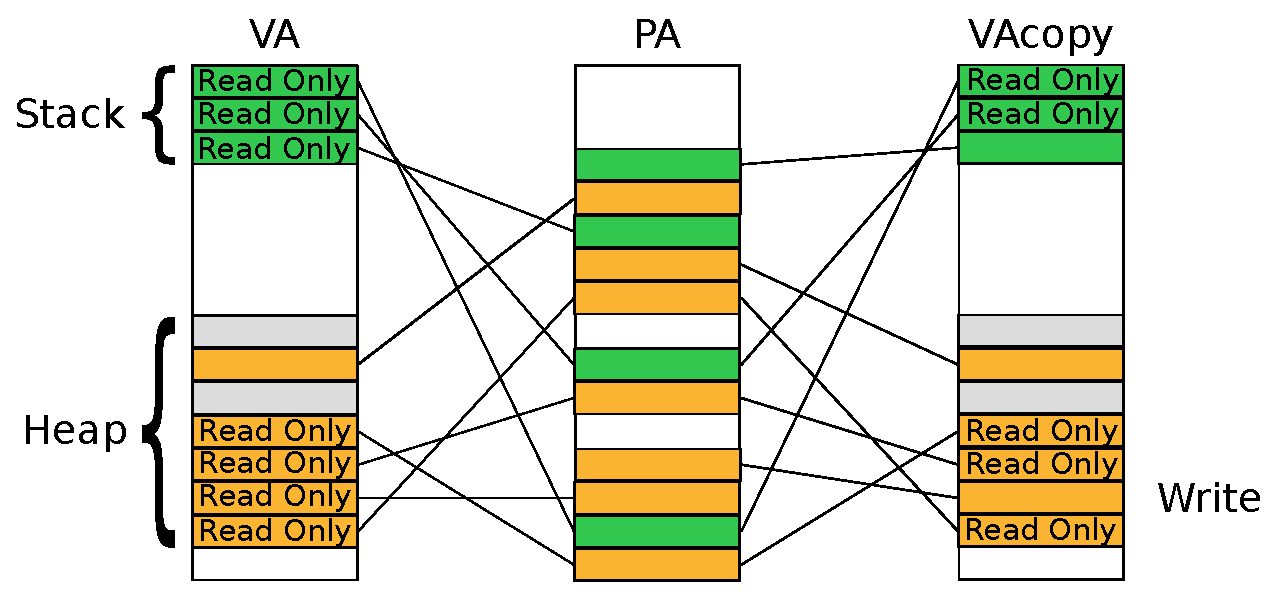
\includegraphics[width=.9\linewidth]{page-cow3}
  \caption{При записи происходит аллокация и настоящее копирование}
\end{figure}
\end{frame}

\begin{frame}
\frametitle{Page Fault}
\framesubtitle{Copy On Write}

\begin{figure}
  \centering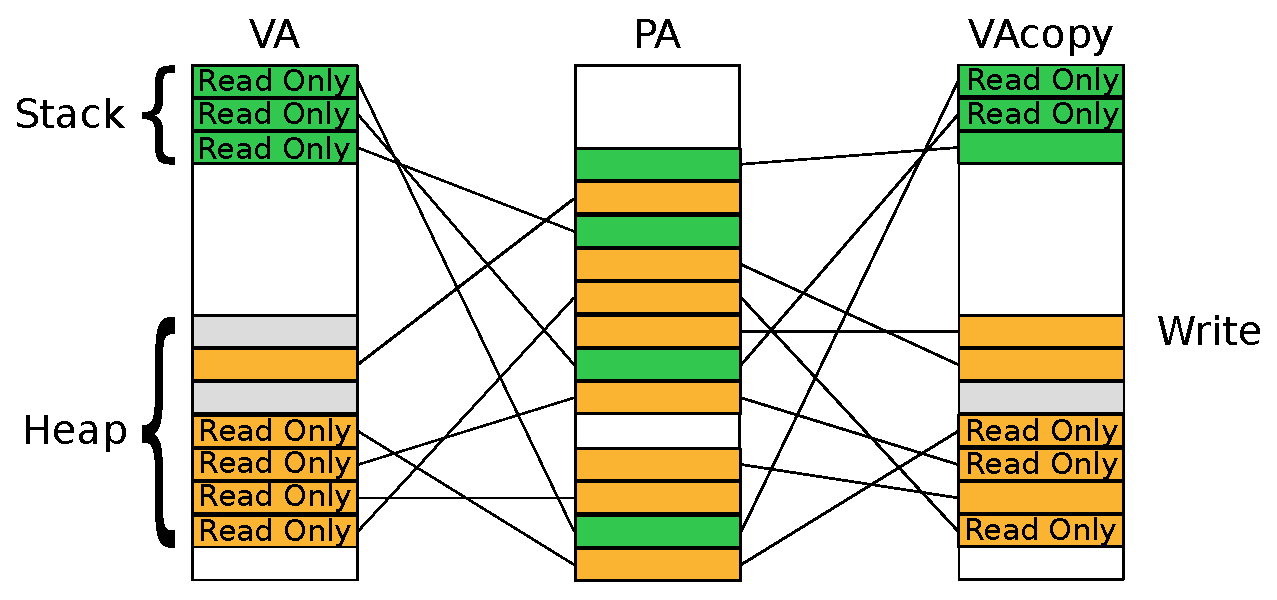
\includegraphics[width=.9\linewidth]{page-cow4}
  \caption{При записи происходит аллокация и настоящее копирование}
\end{figure}
\end{frame}

\begin{frame}
\frametitle{Page Fault}
\framesubtitle{Copy On Write}

Для реализации Copy On Write, кроме наличия Page Fault, еще необходимы:
\begin{itemize}
  \item счетчик ссылок для физических страниц - мы должны знать, что страницу нужно копировать;
    \begin{itemize}
      \item если вы используете Buddy Allocator, то у вас уже есть дескриторы для страниц - в них можно хранить счетчик ссылок;
    \end{itemize}
  \item "предполагаемые" права доступа к странице - мы должны знать, правда ли страница Read Only, или только из-за Copy On Write.
    \begin{itemize}
      \item для каждого процесса должна быть структура описывающая его VA (в Linux Kernel она называется mm\_struct, в FreeBSD она называется vmspace, в MAC OS X она называется vm\_map)
    \end{itemize}
\end{itemize}
\end{frame}

\begin{frame}
\frametitle{Non-Contigous Page Allocation}

\begin{itemize}
  \item<1-> Аллокация больших блоков памяти может провалиться из-за фрагментации.
  \item<2-> Paging позволяет отобразить последовательные участки VA на непоследовательные участки PA.
  \item<3-> Необходимо только иметь участок VA достаточного размера.
\end{itemize}
\end{frame}

\begin{frame}
\frametitle{Адресное пространство процесса}

\begin{columns}[T]
  \begin{column}{.4\textwidth}
    \begin{figure}
      \centering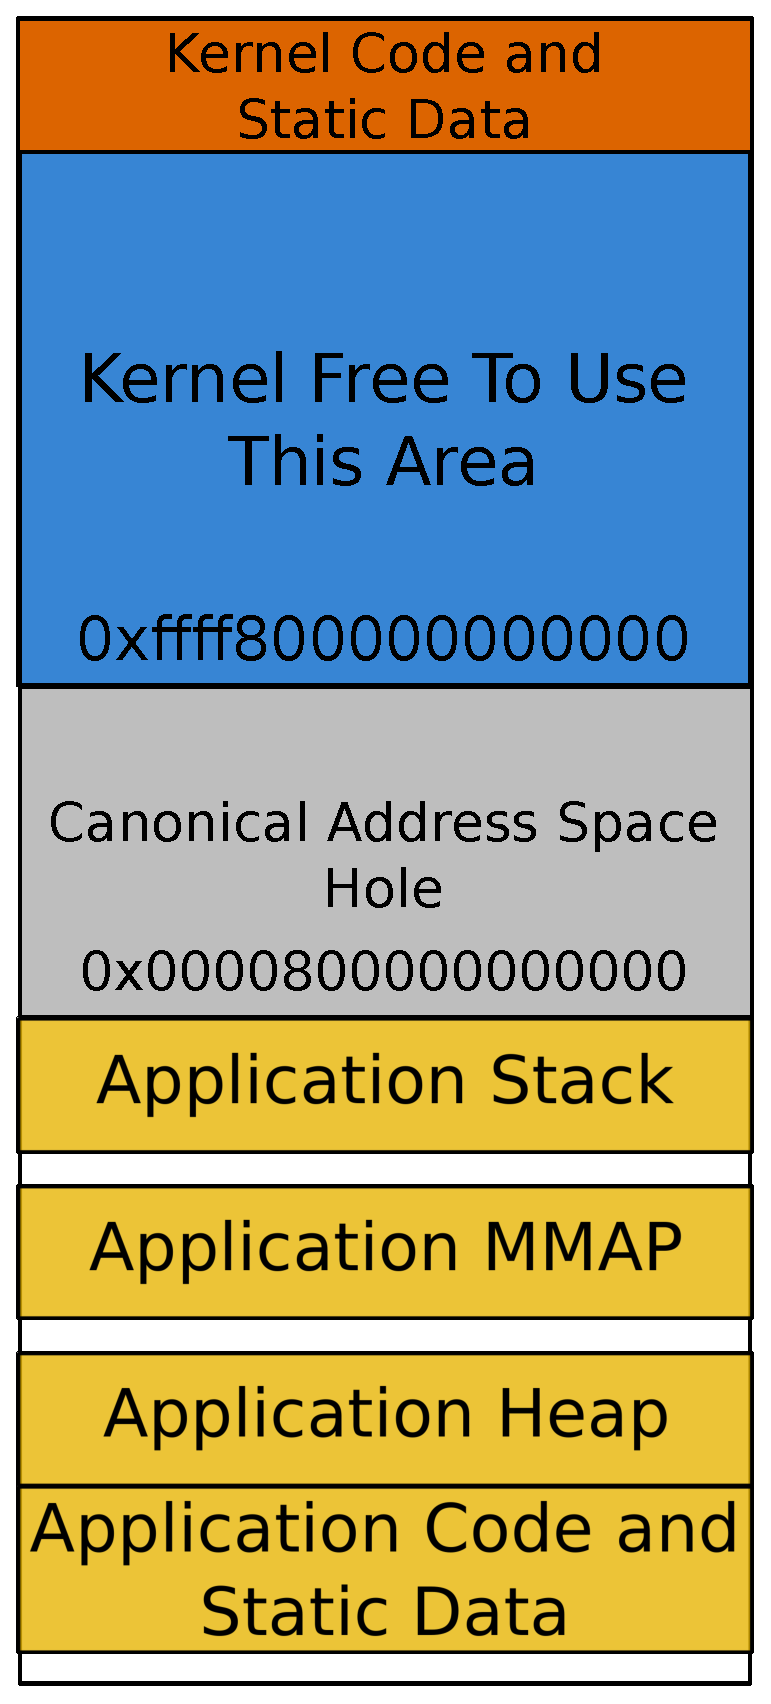
\includegraphics[height=.6\textheight]{memmap}
      \caption{Типичная структура VA на x86-64}
    \end{figure}
  \end{column}
  \begin{column}{.5\textwidth}
    \begin{itemize}
      \item Процессоры Intel поддерживают порядка 2TB RAM.
      \item У нас есть $2^{47} - 2GB$ VA между "дырой" и ядром (по факту, бесконечное VA).
      \item Будем аллоцировать непрерывные участки VA и отображать страницы на них.
    \end{itemize}
  \end{column}
\end{columns}
\end{frame}

\begin{frame}
\frametitle{There is much more about paging}

За кадром остлось много полезных тем:
\begin{itemize}
  \item<2-> использование свободных страниц (коснемся этого когда дойдем до ФС)
    \begin{itemize}
      \item свободная память - бесполезная память;
      \item Page Cache, Buffer Cache, и много других;
    \end{itemize}
  \item<3-> swapping:
    \begin{itemize}
      \item swapping возможен и без Paging-а;
      \item Paging позволяет не выгружать все VA процесса на диск;
    \end{itemize}
  \item<4-> для Linux Kernel есть подробное (немного устаревшее) описание по \href{https://www.kernel.org/doc/gorman/}{ссылке}
\end{itemize}

\end{frame}
